%%%%%%%%%%%%%%%%%%%%%%%%%%%%%%%%%%%%%%%%%%%
\begin{frame}{Codigo}
	\only<1>{
		\begin{figure}
			\centering
			\tiny\lstset{language=python}
			\lstinputlisting[firstline=1,lastline=13]{RW01.py}
		\end{figure}
		}
	\only<2>{
		\begin{figure}
			\centering
			\tiny\lstset{language=python}
			\lstinputlisting[firstline=14,lastline=21]{RW01.py}
		\end{figure}
	}
\end{frame}
%%%%%%%%%%%%%%%%%%%%%%%%%%%%%%%%%%%%%%%%%%%
\begin{frame}{Caminata Aleatoria de $n$  transiciones}
	\begin{overlayarea}{\textwidth}{.7\textheight}
	\only<1>{	
		\begin{center}
			\includegraphics[width=\textwidth]{./IMAGENES/RW/RW01(1).png}	
		\end{center}
	}
	\only<2>{
		\begin{center}
			\includegraphics[width=\textwidth]{./IMAGENES/RW/RW01(2).png}	
		\end{center}	
	}
	\only<3>{
		\begin{center}
			\includegraphics[width=\textwidth]{./IMAGENES/RW/RW01(3).png}	
		\end{center}	
	}	
	\end{overlayarea}
\end{frame}
%%%%%%%%%%%%%%%%%%%%%%%%%%%%%%%%%%%%%%%%%%%%%%%%%%%%%%%%%%%%%%%%%%%%%%%%%
\begin{frame}{Construcci\'on}
	\begin{empheq}[box={\Garybox[Construcci\'on]}]{align*}
		h^{2}&=\delta\\	
		Y_{\delta,h}(t) 
		& \xrightarrow[\delta ,h \to 0]{\mathcal{D}} B(t) \qquad \forall t \geq 0\\
		\mathbb{E}\left[e^{i\lambda B(t)}\right] 
		&
		\xrightarrow{\delta ,h \to 0}
		e^{-\frac{1}{2}t\lambda^{2}}, \quad \lambda \in 	\mathbb{R}.	
	\end{empheq}	
\end{frame}
%%%%%%%%%%%%%%%%%%%%%%%%%%%%%%%%%%%%%%%%%%%%%%%%%%%%%%%%%%%%%%%%%%%%%%%%%%%%%
\begin{frame}{Distribuci\'on Gaussiana}
	\begin{figure}	
		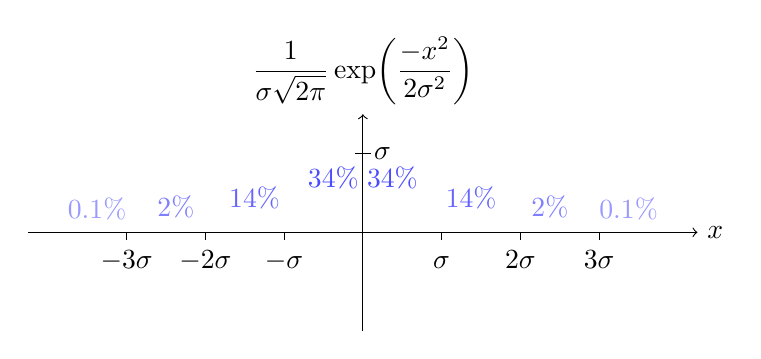
\begin{tikzpicture}[scale=1.0]
    		\colorlet{col1}{blue!70}
		\colorlet{col2}{blue!60}
		\colorlet{col3}{blue!50}
		\colorlet{col4}{blue!40}
   		%\draw [help lines] (-4.25,-1.25) grid (4.25,1.5);
		%\draw [help lines,step=0.25cm] (-2.99,0) grid (2.99,0.99);
		\draw[->] (0,-1.25) -- (0,1.5) node [above]
		{$\displaystyle
			\frac{1}{\sigma\sqrt{2\pi}}\exp\biggl(\frac{-x^2}{2\sigma^2}\biggr)
		$};
		\begin{scope}[smooth,draw=gray!20,y=0.3989422804cm]
        \filldraw [fill=col3] plot[id=f1,domain=-3:-2] function {exp(-x*x/2)}
            -- (-2,0) -- (-3,0) -- cycle;
        \filldraw [fill=col2] plot[id=f2,domain=-2:-1] function {exp(-x*x/2)}
            -- (-1,0) -- (-2,0) -- cycle;
        \filldraw [fill=col1] plot[id=f3,domain=-1:0]  function {exp(-x*x/2)}
            -- (0,0)  -- (-1,0) -- cycle;
        \filldraw [fill=col1] plot[id=f4,domain=0:1] function {exp(-x*x/2)}
            -- (1,0)  --  (0,0) -- cycle;
        \filldraw [fill=col2] plot[id=f5,domain=1:2] function {exp(-x*x/2)}
            -- (2,0)  -- (1,0) -- cycle;
        \filldraw [fill=col3] plot[id=f6,domain=2:3] function {exp(-x*x/2)}
            -- (3,0)  -- (2,0) -- cycle;
        \draw[black] plot[id=f7,domain=-4.25:4.25,samples=100]
            function {exp(-x*x/2)};
		\end{scope}
       \draw[->] (-4.25,0) -- (4.25,0) node [right] {$x$};
    \foreach \pos/\label in {-3/$-3\sigma$,-2/$-2\sigma$,-1/$-\sigma$,
            1/$\sigma$,2/$2\sigma$,3/$3\sigma$}
        \draw (\pos,0) -- (\pos,-0.1) (\pos cm,-3ex) node
            [anchor=base,fill=white,inner sep=1pt]  {\label};

    \draw (-0.1,1) -- (.1,1) node [right,fill=white,inner sep=1pt] {$\sigma$};

    \foreach \pos/\percent/\height in {1/34/0.5,2/14/0.25,3/2/0.125,4/0.1/0.1}
    {
      \node[text=col\pos,anchor=base,yshift=2pt,xshift=-0.625cm,
        fill=white,inner sep=1pt] at (\pos,\height) {$\percent\%$};
      \node[text=col\pos,anchor=base,yshift=2pt,xshift=.625cm,
        fill=white,inner sep=1pt]  at (-\pos,\height) {$\percent\%$};
    }
	\end{tikzpicture}
	\end{figure}
\end{frame}
%%%%%%%%%%%%%%%%%%%%%%%%%%%%%%%%%%%%%%%%%%%%%%%%%%%%%%%%%%%%%%%%%%%%%%%%%%
\begin{frame}{Caminata Aleatoria en $[0,1]$}
	\vspace{-1.5cm}		
	\begin{overlayarea}{\textwidth}{.7\textheight}
	\only<1>{	
		\begin{center}
			\includegraphics[width=\textwidth]{./IMAGENES/RW/RWs01.png}	
		\end{center}
	}
	\only<2>{
		\begin{center}
			\includegraphics[width=\textwidth]{./IMAGENES/RW/RWs01Sigma.png}	
		\end{center}	
	}
	\end{overlayarea}
\end{frame}



